\chapter{Hardwareumsetzung}
\label{cha:robot}
\section{Entwurf des NXT-Roboters}

Der Roboter hat einige hardwareseitigen Voraussetzungen. Das System muss sich frei im Raum bewegen können, sowie eine Möglichkeit bieten mit Gegenständen zu interagieren. Diese müssen aufgehoben, transportiert und zielgerichtet abgelegt werden können. Es ist zusätzlich wichtig, dass die Gegenstände beim Ablegen sicher an ihrer Position verharren, damit sie sich nicht aus einer möglichen Zielzone heraus bewegen. Wichtiges Kriterium ist zusätzlich eine sichere Halterung für das Kameramodul, welches in Kapitel \ref{sec:Kamera} näher beschrieben ist.

Da das LEGO Mindstorm NXT Kit häufig zur Realisierung kleinerer Roboterprojekte verwendet wird, hat LEGO eine Datenbank an möglichen Bauplänen bereitgestellt \cite{building_instructions}. Nach einiger Recherche und Durchsicht diverser Bauanleitungen für verschiedenste Anwendungsbereiche wurde sich für einen von LEGO bereitgestellten Aufbau den entschieden. Abbildung \ref{fig:standardRoboter} zeigt den Roboter, wie LEGO ihn bereitstellt.

\begin{figure}[h]
\centering
\todo{Bild von Standard Roboter einfügen}
\caption{Von Lego bereitgestellter Roboteraufbau}
\label{fig:standardRoboter}
\end{figure}


Da der Aufbau jedoch nicht allen Anforderungen genüge tut, wurde dieser abgeändert.

Sie wurde lediglich um den Schall- und den Abstandssensor erleichtert; eine Halterung für das Smartphone wurde hinzugefügt.

\todo{hier Bild des Roboters einfügen}

\pagebreak

\subsection{NXT-Stein}

\begin{figure}[h]
\centering
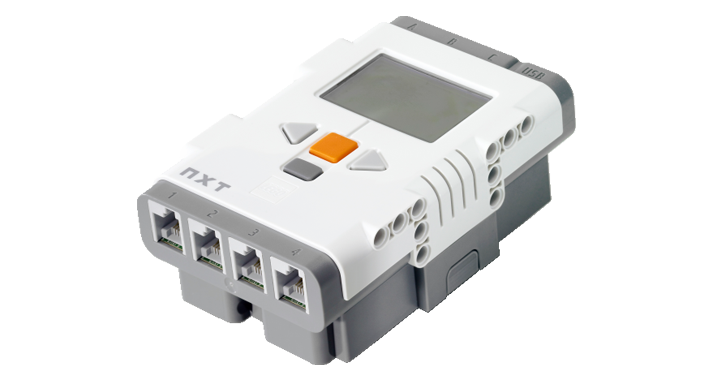
\includegraphics[width=0.5\textwidth]{Bilder/Robot/nxt_brick}
\caption{NXT-Stein}
\label{fig:nxtBrick}
\end{figure}

Der NXT-Stein bildet die Recheneinheit und damit die Hauptkomponente des NXT-Robotersystems. Er besitzt oben drei Ausgänge für Motoren über die gleichzeitig die Rotationssensoren in den Servo-Motoren ausgelesen werden.

Unten befinden sich vier Eingänge für verschiedene Sensoren, die je nach Anwendungszweck über Flachbandkabel bestückt werden können, etwa ein Licht-, Schall-, Tastsensor oder beliebige Kombinationen daraus. Dies macht das NXT-System zu einem sehr flexiblem da einfach konfigurierbaren Robotersystem.

Über einen USB-Anschluss oben wird der NXT mit dem PC verbunden um ihn mit Programmen zu versorgen. Hierfür wird von LEGO eine graphische Entwicklungsumgebung bereitgestellt um auch Neulingen den Einstieg in die Roboter-Programmierung zu vereinfachen und ihnen die Möglichkeit zu bieten schon innerhalb weniger Minuten einen funktionierenden Prototypen auf die Beine stellen zu können. Im Fall des CLEEN-R-Aufbaus wird jedoch lediglich die interne Bluetooth-Verbindung genutzt.

Vorne befindet sich ein 100 mal 64 Pixel auflösendes binäres LCD-Display über das Einstellungen getätigt oder Statusmeldungen ausgegeben werden können. Auch Sound-Ausgabe über einen integrierten 8-Bit-Lautsprecher ist möglich.

\subsection{Sensoren}

\subsubsection{Tastsensor}

\begin{figure}[h]
\centering
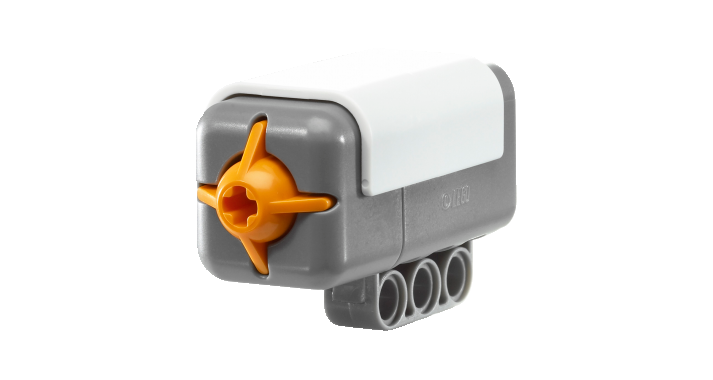
\includegraphics[width=\textwidth/3]{Bilder/Robot/button_sensor}
\caption{Tastsensor des NXT-Systems}
\label{fig:buttonSensor}
\end{figure}

Der berührungsempfindliche Sensor vorne diente zum Detektieren von Gegenständen im Bereich des Greifarms, woraufhin dieser geschlossen werden kann. Er wurde durch den Ultraschallsensor ersetzt, der nicht nur die unmittelbare Berührung bemerkt sondern auch ein herannahendes Objekt während der Fahrt detektiert.

\subsubsection{Rotationssensoren}

Die Rotationssensoren in den Servomotoren erlauben es dem NXT-Roboter, die Geschwindigkeit der Motoren abhängig des Widerstands (des Untergrunds) zu regulieren. So werden unter anderem präzises Abbremsen und Fehlerminimierung bei der Positionsbestimmung ermöglicht.

\subsubsection{Farbsensor}

\begin{figure}[h]
\centering
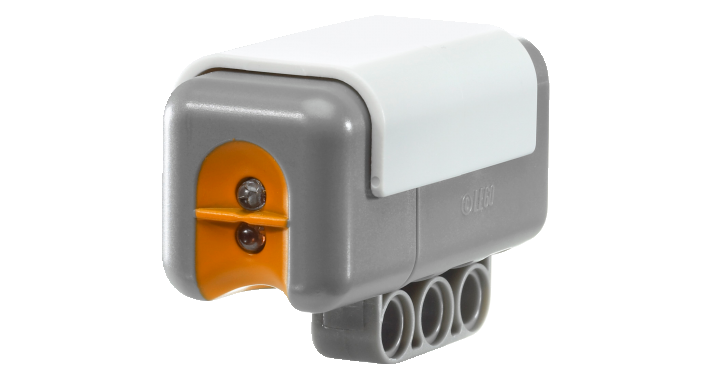
\includegraphics[width=\textwidth/3]{Bilder/Robot/color_sensor}
\caption{Farbsensor des NXT-Systems}
\label{fig:colorSensor}
\end{figure}

Der RGB-Sensor am Boden des NXT dient dazu, die Farbe des Bodens herauszufinden. Diese kann sowohl dazu genutzt werden, bei der Bildverarbeitung die Hintergrundfarbe herauszurechnen und so die Qualität der Objekterkennung zu erhöhen, als auch eine farblich markierte Zielzone im Raum finden zu können, auf der ein getragenes Objekt abgelegt werden kann.

\subsubsection{Ultraschallsensor}
\label{subsec:Ultraschall}

\begin{figure}[h]
\centering
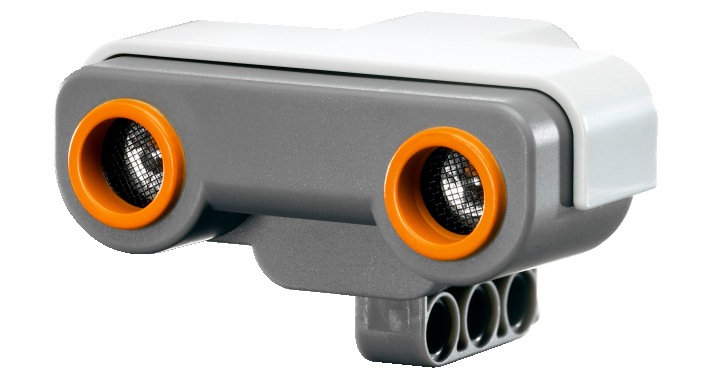
\includegraphics[width=\textwidth/3]{Bilder/Robot/distance_sensor}
\caption{Ultraschallsensor des NXT-Systems}
\label{fig:distanceSensor}
\end{figure}

Der Ultraschallsensor dient zur Messung der Distanz vom Roboter zum nächsten soliden Objekt. Hier wird er genutzt um zu detektieren, wie weit ein Objekt vom Greifarm entfernt ist, um diesen im geeigneten Moment zu schließen und so das Objekt mitnehmen zu können. Auch ermöglicht er ein geregeltes Heranfahren an ein Objekt. Die Präzision des Distanzsensors beträgt $\pm$3cm.

\subsection{Aktoren}

\subsubsection{Antriebsmotoren}

\begin{figure}[h]
\centering
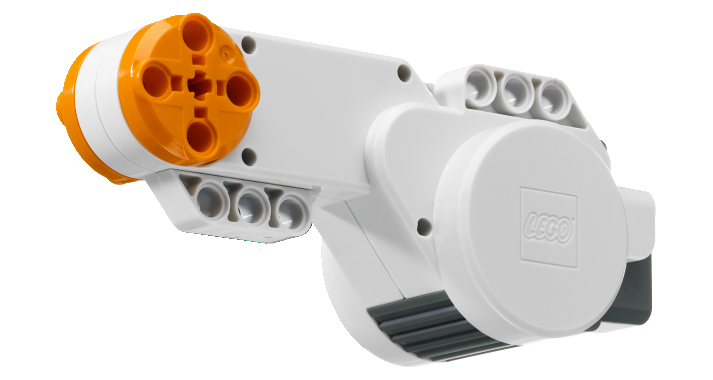
\includegraphics[width=\textwidth/3]{Bilder/Robot/motor}
\caption{Servo-Motor des NXT-Systems}
\label{fig:motor}
\end{figure}

Die beiden Servomotoren links und rechts des NXT-Roboters bilden den differentialen Antrieb und ermöglichen freie Fortbewegung.

\subsubsection{Greifarmmotor}
\label{greifarm}
Der dritte Motor im vorderen Teil des Roboters dient zum Öffnen und Schließen des Greifarms und so zur Mitführung von Gegenständen.

\section{Steuerung des Roboters}

Die Steuerung des Roboters durch das Smartphone erfolgt via Bluetooth. Der NXT-Roboter stellt hierzu als Bluetooth-Gerät das Serial Port Profile (SPP) bereit, welches quasi das Standardinterface auf Bluetooth-Ebene darstellt und vom Großteil aller Bluetooth-Hostgeräte unterstützt wird. Es ermöglicht das simple serielle Senden und Empfangen von Bytes auf Low-Level-Ebene.

Das Kommunikationsprotokoll auf High-Level-Ebene und damit die nötigen Befehle zum Regeln der Aktoren und Auslesen der Sensoren wurde von LEGO dokumentiert und ist online erhältlich\cite{nxt_comm_protocol}.

\begin{figure}[h]
\centering
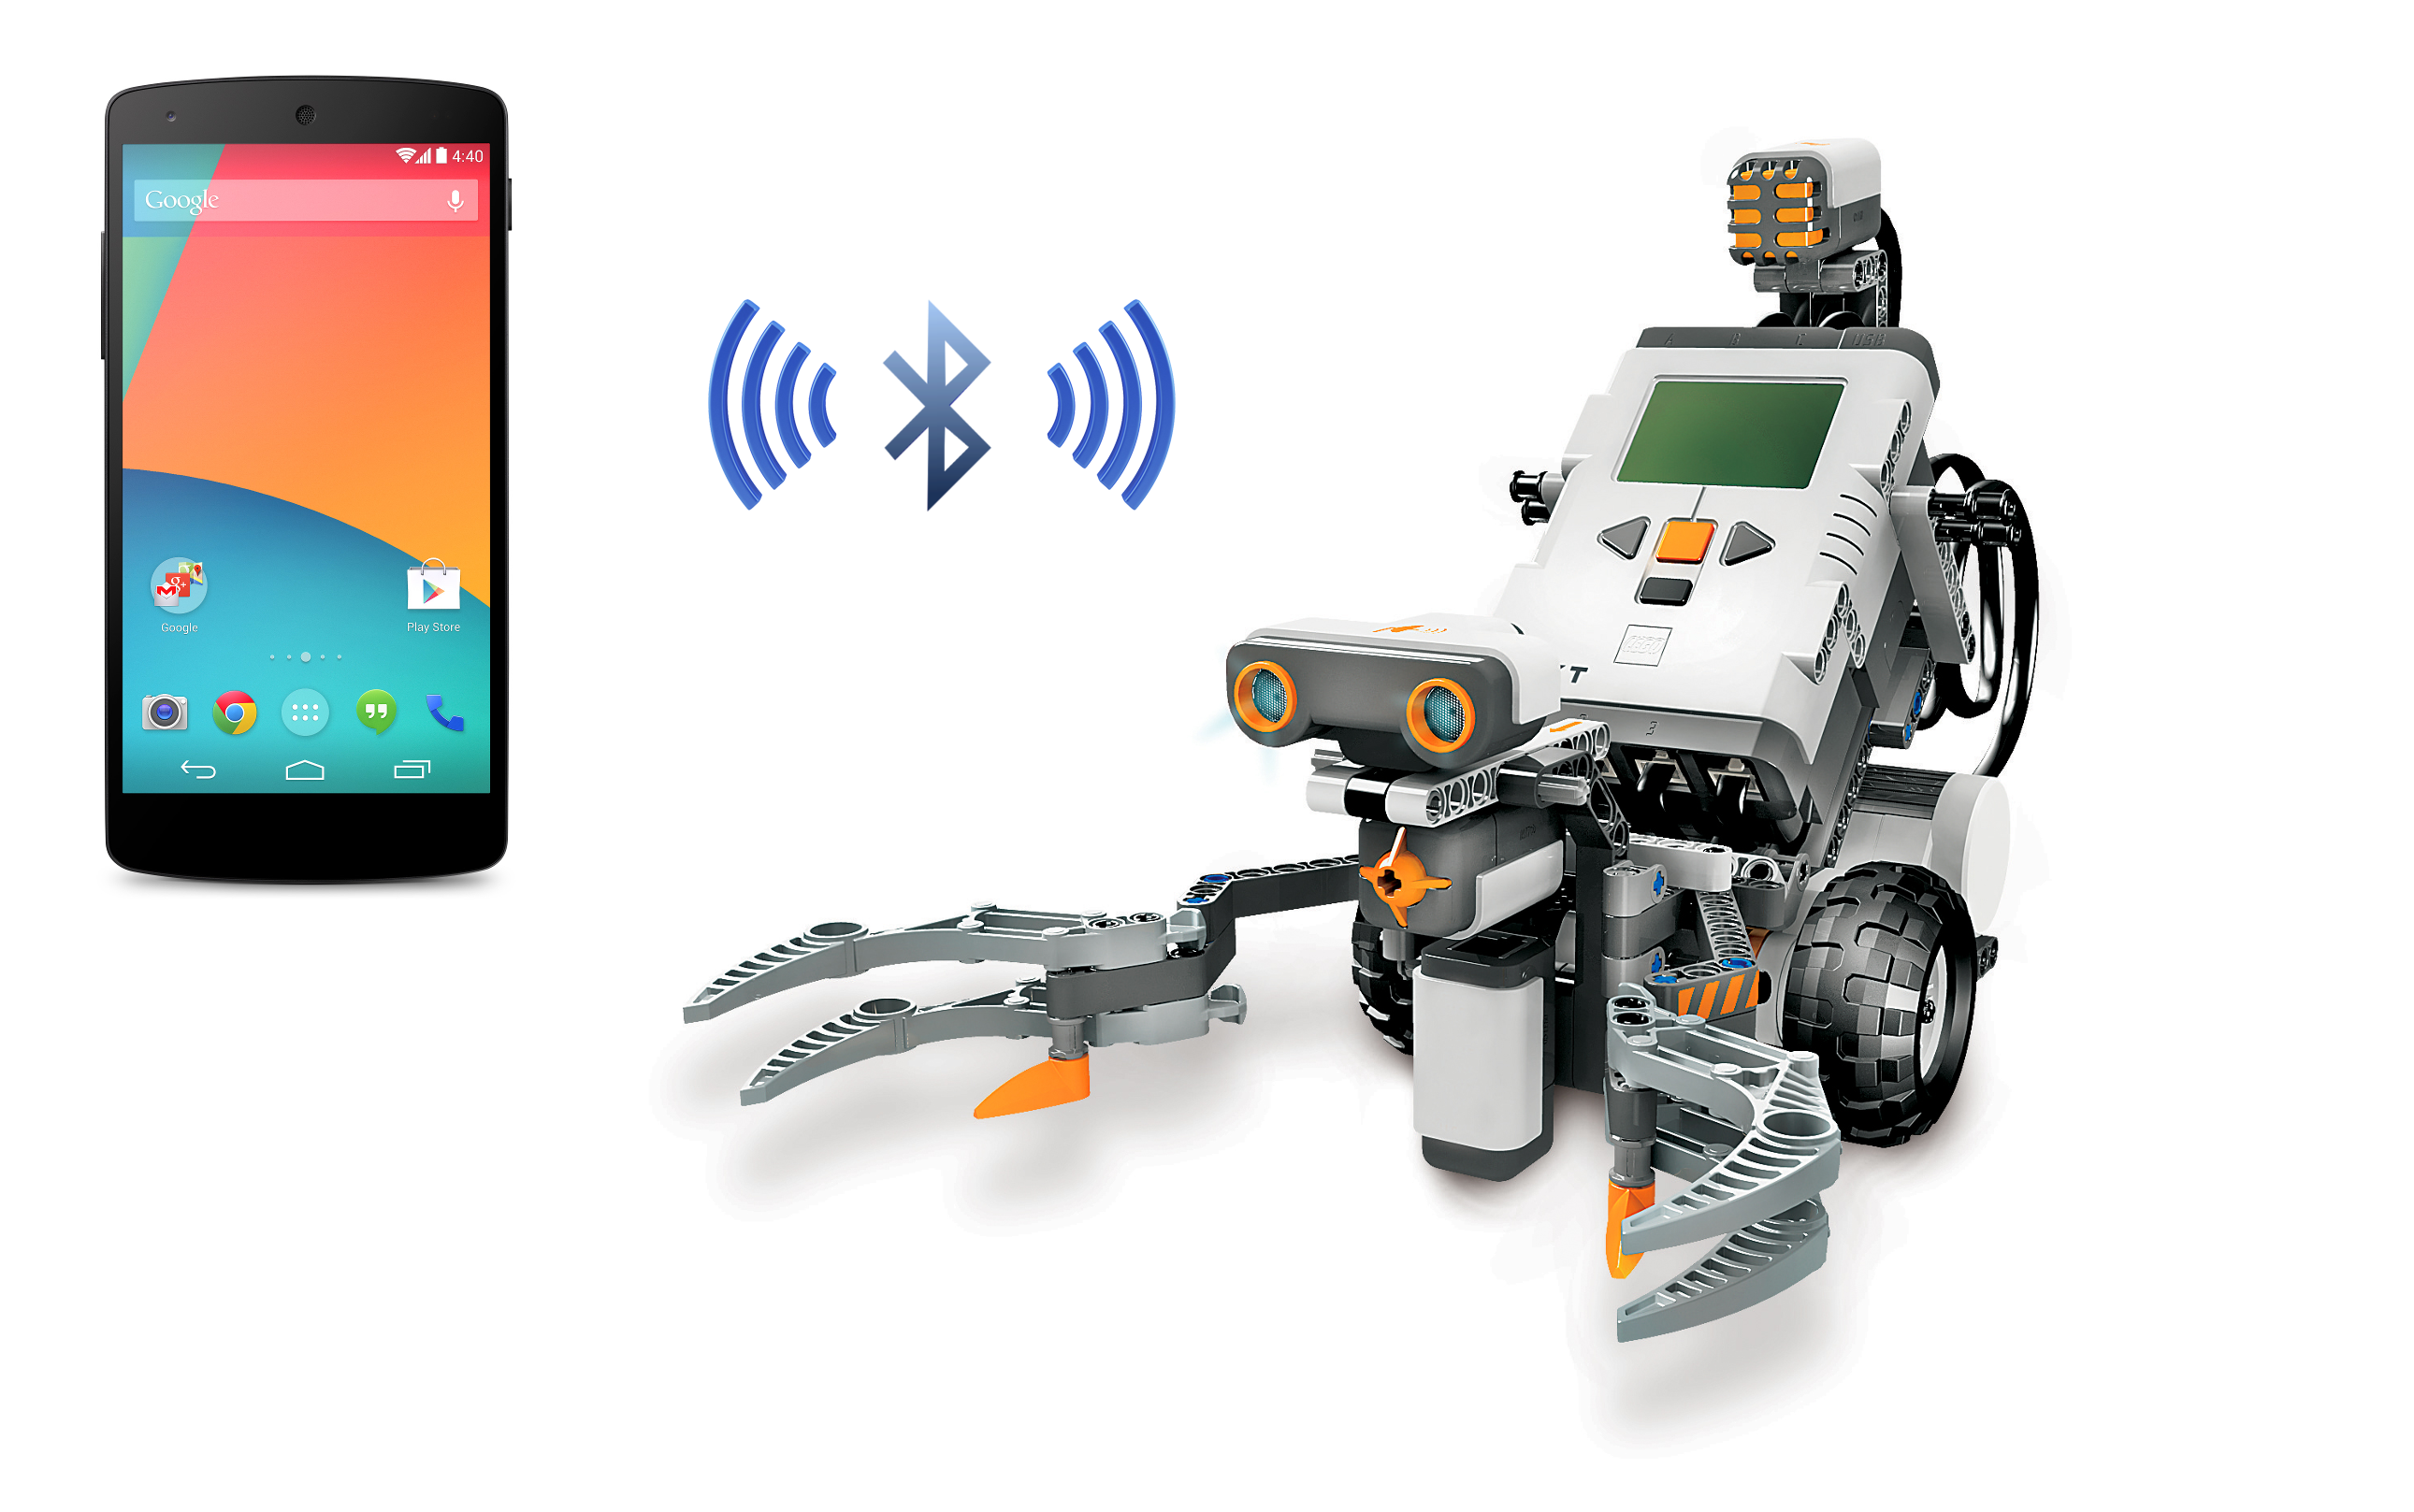
\includegraphics[width=\textwidth/2]{Bilder/Robot/bluetooth}
\caption{Bluetooth-Verbindung zwischen NXT und Nexus 5}
\label{fig:bluetooth}
\end{figure}

Auf dem NXT selbst wird hierbei kein Programm ausgeführt, um alle Logik zentral in der NXT-App auf dem Smartphone zu halten.

Zunächst muss eine Bluetooth-Verbindung erstellt werden, wozu beide Geräte aktiviertes Bluetooth aufweisen, der Roboter zusätzlich sichtbar für das Smartphone sein müssen.

Bei Erstverbindung muss der gesuchte NXT ausgewählt werden, danach ist die Bluetooth-Adresse bekannt und die App kann ohne Benutzerinteraktion eine Verbindung mit dem NXT-Roboter aufnehmen.

Kommt eine Verbindung zustande, können seriell Byte für Byte die Kommandos an den NXT übertragen, eventuelle Antworten empfangen werden.

App-seitig übernimmt ein gesonderter Thread in der Klasse NxtTalker nach Zustandekommen einer Verbindung das Management der Daten.

Zum Bewegen der Motoren muss zunächst per Befehl pro Aktor eine Geschwindigkeit im Bereich von -100\% bis 100\% (und Parameter wie Regulierung) übergeben, zum Stoppen können alle Motoren mit einem Befehl auf Geschwindigkeit '0' gesetzt werden.

Zwei Motoren können synchronisiert werden, sodass diese gleichzeitig starten. Ansonsten würde der Zeitversatz zwischen dem Absetzen der zwei 'setze Geschwindigkeit'-Befehle bewirken, dass der Roboter vor dem geradeaus fahren kurz nur das erste Rad ansteuert und in eine Richtung abdriftet.

